\documentclass[a4paper,12pt, twoside]{book}

\pagestyle{myheadings}
\usepackage{blindtext}

\usepackage{geometry}
\usepackage{newtxmath,newtxtext}
\usepackage{ragged2e}
\usepackage{indentfirst}
\usepackage{titlesec}
\usepackage[utf8x]{inputenc}
\usepackage[romanian]{babel}
\usepackage{combelow}
\usepackage{newunicodechar}
\usepackage{graphicx}
\graphicspath{ {./Diagrams/} }

\newunicodechar{Ș}{\cb{S}}
\newunicodechar{ș}{\cb{s}}
\newunicodechar{Ț}{\cb{T}}
\newunicodechar{ț}{\cb{t}}
\newunicodechar{ă}{\u{a}}

\geometry{
	top 	= 3.5cm,
	bottom 	= 3cm,
	inner 	= 3cm,
	outer 	= 2cm,
	bindingoffset=0cm,
	headsep = 0.5cm,
	headheight = 0.5cm,
	footskip = 1cm,
}
\title{Lucrare Licenta}
\author{Steleac Raul-Dacian}

\titleformat{\chapter}
{\normalfont\fontsize{20}{14}\bfseries\sffamily}{\thechapter}{1em}{}
\titleformat{\section}
{\normalfont\fontsize{16}{14}\bfseries\sffamily}{\thesection}{1em}{}
\titleformat{\subsection}
{\normalfont\fontsize{14}{14}\bfseries\sffamily}{\thesubsection}{1em}{}

\titlespacing{\chapter}{0cm}{00pt}{30pt}
\titlespacing{\section}{0cm}{40pt}{20pt}
\titlespacing{\subsection}{0cm}{20pt}{10pt}

\let\OLDthebibliography\thebibliography
\renewcommand\thebibliography[1]{
	\OLDthebibliography{#1}
	\setlength{\parskip}{0pt}
	\setlength{\itemsep}{0pt plus 0.3ex}
}

\begin{document}
	\maketitle
	\thispagestyle{empty}
	\tableofcontents
	\thispagestyle{empty}
	\clearpage
	\thispagestyle{empty}
	
	\chapter{Introducere generala}
	
		\section{Prezentarea Problemei}
						
			\setlength{\parindent}{0.8cm}
			
			Comunicarea este o capacitate esențială pentru specia umană, fiind cel mai natural si principalul mod de transmitere a informației într-un mod direct. Totuși pe lângă informația lingvistică o mare parte din informațiile prezente în conversațiile pe care le avem zilnic sunt ascunse în emoțiile cu care rostim și articulăm diferite cuvinte, silabe și chiar litere. Urechea umană este capabilă să determine și cele mai mici inflexiuni din vocile participanțiilor la conversație pentru a reuși să capteze cât mai bine sensul acesteia. Astfel, e de așteptat că mașinile care urmează să facă parte de acum din aceste conversații să fie la fel de competente din aceasta privința. Domeniul stintific care se ocupă cu crearea unor modele de tip "Machine Learning" pentru determinarea emoțiilor dintr-un discurs se numește "Speech Emotion Recognition", sau SER. \par	
			
			\subsection{Importanta Informatiei Emotionale}	
				In trecut, majoritatea studiilor legate de rolul emotiei umane in acustica 	unui discurs au fost facute in psihologie. Blanton \cite{blanton}, de exemplu, a scris ca "efectul emotiei asupra intonatiilor vocii sunt recunsocute de orice persoana. Chiar si cele mai primitive specii pot recunoaste tonuri care reprezinta dragoste, frica sau enervare. Cainii, caii, si multe alte animale pot intelege parti din limbajul uman. Limbajul tonurilor este cel mai vechi si universal dintre toate modurile de comunicare".\par 
				Putem astfel sa ne gandim la modurile de comunicare pe care stramosii nostri le foloseau inainte de inventarea cuvintelor. Capacitatea obtinerii unei forme de limbaj nu era posibila pentru specia \textit{Homo erectus}, stramosii speciei \textit{Homo sapiens}, deoarece dezvoltarea vorbirii a necesitat o conexiune directa a cortexului motor central cu muschii intercostali , conexiune care lipseste din constructia coloanei vertebrale ale speciei \textit{Homo erectus}. Levinson \& Holler \cite{leviholler} sustin conventia ca limbajul a aparut cu aproximativ o suta de mii de ani dupa aparitia speciei umane, care se estimeaza a fi acum circa trei sute de mii de ani. Se considera astfel ca a existat o perioada de circa o suta de mii de ani in care stramosii nostri, \textit{Homo sapiens}, desi capabili sa folosesaca un limbaj pentru comunicare, nu au facut-o. Christiansen \& Kirby \cite{chriskirbi} mentioneaza un consens intre cercetatorii acestui domeniu in legatura cu pasii necesari prin care o specie poate sa dezvolte un limbaj. Mai exact, consensul este ca inainte de aparitia limbajului cateva "pre-adaptari" au trebuit sa apara in descendentii familiei \textit{Hominidae}. Desi cercetatorii nu sunt complet de acord in legatura cu lista acestor "pre-adaptari", un candidat propus de majoritate a fost abilitatea de folosi asa numite "simboluri". In acest context, aceste simboluri reprezinta capacitatea de a crea legaturi intre sunete si gesturi arbitrare cu anumite concepte sau perceptii specifice. Gesturi si suntete arbitrare erau suficiente pentru a exprima diferite emotii ca fericire, frica, intristare sau manie, consolidand astfel bazele comunicarii care a oferit oamenilor avatajul evolutiv. Putem sa obesrvam cum desi informatia lingvistica nu exista inca in comunicarea speciei umane, informatia emotionala a fost inclusa inca de la primele forme de interactiuni sociale.\par 
				Cantitatea de informatie din spatele emotiilor pe care le folosim astazi in limbajul modern ramane fel de importanta ca pe vremea stramosilor nostri. De aceea, in prezent, studiul importantei emotiei dintr-o conversatie este extins si in domeniul calculatoarelor prin inteligenta artificiala. \par	
			\subsection{Prezentare SER}
				Domeniul "Speech Emotion Recognition", sau SER, are ca scop final construirea unui model de tip "Machine Learning" care sa primeasca de la intrare o inregistrare audio, reprezentand o parte dintr-o conversatie, si sa genereze la iesire o emotie, care sa fie reprezentativa pentru acea inregistrare. \par
				Recunoasterea emotiilor in vorbire este o problema care a starnit curiozitatea adeptilor domeniului inteligentei artificiale de cateva decenii. Daellert et al. \cite{dellaert} au deschis granitele acestui domeniu in 1996 cu primul articol stintific care incearca sa combata acest subiect. Acestia au incercat sa clasifice patru tipuri de emotii prin folosirea unor date de intrare asa numite "prosodice" ca tonalitatea, intensitatea, frecventa sau amplitudinea folosind trei tipuri de modele diferite "Maximum Likelihood Bayes classifier" (MLB), "Kernel Regression"  (KR) si "K-nearest neighbors" (KNN). Aceasta implementare este una reprezentativa pentru combaterea recunoasterii de emotii in vorbire, realizand o separare clara intre cele doua module arhitecturale principale: extragerea datelor si clasifiactorul care urmeaza sa fie antrenat. Discrepanta dintre arhitecturile folosite in prezent si cea prezentata mai sus ramane insa observabila. Chiar daca datele de intrare prosodice sunt inca folosite astazi, cresterea drastica a puterii de procesare a dus la folosirea unor arhitecturi cu retele neuronale adanci care folosesc ori mai multe tipuri de date de intrare ori direct semnalul audio neprocesat, daca modelul realizeaza extragerea datelor printr-o maniera automata, "end-to-end models". \par		
				
				Diferentele arhitecturale sunt totusi un semn benefic, fiind reprezentative pentru evolutia domeniului de cercetare. SER si-a pastrat popularitatea in ultimele doua decenii detinand un numar bogat de articole stintifice pe aceasta tema. Aceste articole aduc noi interpretari atat din punctul de vedere al extragerilor caracteristicilor semnalului audio folosite ca date de intrare cat si a modelului folsoit pentru antrenare. Totusi, desi noi idei si arhitecturi contiuna sa apara anual, aceasta tehnologie nu a reusit sa atinga inca o acuratete destul de satisfacatoare pentru a fi lansata pe piata. \par
					
				Desi, in prezent, recunoasterea emotiei vorbitorilor nu este folosita la potentialul maxim, alte tehnologii asemanatoare ca "Speech Recognition", care incearca sa determine informatia lingvistica dintr-o conversatie, au revolutionat interfetele de comunicare dintre om si masina. Aceasta tehnologie isi gaseste locul in majoritatea telefoanelor, calculatoarelor, masinilor si chiar a unor echipamente din jurul casei. Alexa, Cortana si Siri sunt cateva nume pe care majoritatea persoanelor le cunosc fara sa le asocieze cu o fata sau o persoana. Acesti agenti inteligenti obtin rezultate exceptionale in capacitatea lor de a mentine o conversatie cu clientii, de a raspunde la anumite cerinte ale acestora dar si de a pastra calitatea acelei conversatii la un nivel apropiat de cel uman prin diferite glume sau intonatii cu tenta umoristica sau empatica. \par				
				Pentru a obtine o inerfata de comunicare om-masina de capacitate maxima, informatia emotionala este totusi esentiala. Prin diferite intonatii sensul cuvintelor poate fi schimbat complet iar un algoritm care se focuseaza doar pe informatia lingvistica va ramane inflexibil la aceste intonatii generand astfel rezultate eronate. Chiar daca cele doua domenii de cercetare sunt inrudite din punctul vedere al provocarii pe care incearca sa o rezolve, cele doua sunt diferite in dificulatiile care apar in crearea unui model. Daca pentru "Speech recognition" bazele de date sunt usor de accesat, de exmplu diferite inregistrari impreuna cu varianta tiparita a discursului, pentru "Speech Emotion Recognition" obtinerea bazelor de date reprezinta unul din cele mai mari obstacole.\par
					

		\section{Motivatia Problemei}
			Recunoasterea emotiei in vorbire reprezinta un subiect extrem de interesant atat din punct de vedere aplicativ cat si personal. Potentialul acestui subiect este ridicat din cauza numarului ridicat de aplicatii, modurile in care sistemele SER pot fi utilizate fiind limitate doar de nivelul tehnologic curent.
			\subsection{Motivatie aplicativa}				
					Aplicatiile in care aceasta tehnologie poate fi folosita in viitor sunt greu de estimat, deoarece orice interfata om-masina care se foloseste de vorbire ca transmitere de informatii si comenzi necesita un astfel de algoritm. Cu toatea acestea diferite aplicatii din prezent sunt succeptibile la a fi imbunatatite prin intermediuli introducerii unui model SER. \par
					
					Un bun exemplu este introducerea unui algoritm SER in departamentul de \textbf{"feed-back"} al unei firme. Principala modalitate prin care firmele din zilele noastre incearca sa capteze parerea publicului asupra unui produs este prin folosirea unor chestionare. Chiar daca acestea iau loc in scris sau telefonic, aduc anumite limitari. In prima situatie apare incertitudinea onestitatii oamenilor care raspund iar in cea de a doua situatie apare limitarea personalului disponibil care sa asculte raspunsurile intervievatiilor in decursul chestionarului. Un algoritm de "speech emotion recognition" impreuna cu unul generic de "speech recognition" pot capta atat informatia lingvistica cat si cea emotionala din raspunsurile la chestionar astfel notand atata cuvintele in sine cat si un grad de credibilitate bazata pe implicarea emotionala a participantului. \par
		
					Un alt exemplu ar fi implementarea modelelor SER in arhitecturi care sunt deja folosite pentru comunicarea cu oamenii. Agentii inteligenti si diferitele tipuri de roboti, Huahu et al. (2010) \cite{huahu}, care apar tot mai des in prezent in apropierea oamenilor pot gasi un mare avantaj in determinarea emotiilor clientilor pentru a raspunde cat mai exact la nevoile acestora. De exemplu un agent inteligent incorporat intr-o masina poate detecta daca in timpul mersului soferul este implicat intr-o cearta sau o discutie cu un puternic impact emotional si sa il indrume pe acesta sa opreasa masina pana cand discutia s-a terminat pentru evitarea unui accident din cauza lipsei de atentie. Alexa sau Siri, care sunt folosite de mii de oameni in jurul globului in jurul casei, pot sa incerce sa ofere raspunsuri care sa linisteasca un client nervos sau sa introduca mici glume pentu a incerca sa inveseleasca un client trist. Aplicatiile pentru astfel de agenti inteligenti arata importanta unui model SER in orice interfata de comunicare om-masina, pentru ca le ofera acestora capacitatea de a tine pasul cu emotiile prezente in conversatie, astfel aducand acea comvorbire la un nivel foarte apropiat de cel de la om la om. \par 
						
					Acesti alogritmi ar putea fi folositi si pentru a eficientiza educatia. Prin introducerea unor receptoare de emotii profesorii pot determina starea emotionala a studentiilor si pot extrage informatii pentru imbunatatirea calitatii orelor de curs. De exemplu profesorul poate folosi modelul de recunoastere a emotiilor pentru determinarea continua a interesului studentiilor sau pentru a crea strategii care sa ridice moralul clasei cand vine vorba de anumide subiecte predate care ii pot descuraja sau plictisi pe acestia. \par
					
					Alte exemple care merita mentionate sunt folosirea acestor tipuri de algoritmi in: statii de call center (Gupta and Rajput, 2007 \cite{gupta}), jocuri video ( Szwoch and Szwoch, 2015 \cite{szwoch}), evaluare pshiologica ( Lancker et al., 1989; Low et al., 2011 \cite{lancker} ) etc. Dupa cum putem observa recunoasterea emotiilor poate fi aplciata la orice arhitectura care implica comunicarea cu oamenii, acest orizont fiind limitat doar de imaginatia dezvoltatorilor de tehnologii. \par				
			\subsection{Motivatie Personala}				
					Tema recunoasterii de emotii a inceput sa ma intrige cand mi-am pus problema construirii unui psiholog artificial. Desi un astfel de terapist este putin probabil, recunoasterea de emotii a ramas o problema cu potentialul de a fi rezolvata. In subiecte ca recunoasterea obiectelor, fetelor, si chiar a cuvintelor rostite s-a obtinut o acuratete destul de satisfacatoare pentru a fi introduse pe piata. Pentru SER acest aspect nu este valabil inca. \par
					Detectarea emotiilor m-a pasionat din cauza ca deschide noi oportunitati in capacitatea de comunicare existenta intre om si masina. Emotile umane si relatiile dintre ele si stimulii externi nu sunt intelese inca in mod complet, astfel studiul SER din punctul de vedere al intelgentei artificiale are potentialul sa descopere noi intelesuri legate de modul de formare al emotiilor umane. \par
					\hfill \par
					--------- add stuff ----------
			\section{Obstacole in studiul SER}			
				Principalele probleme care despart SER de majoritatea aplicatiilor de "Machine Learning" sunt legate de dificultatea obtinerii unui set de date de intrare satisfacator comparativ cu complexitatea problemei si lipsa unor caracteristici de intrare care sa fie reprezentative pentru detectarea emotiei.\par
				
				Aceste doua considerente au alcatuit in decusul ulitmelor doua deceni obstacole serioase in studiul si dezvoltarea modelelor de recunoastere de emotii deoarece implica necesitatea folosirii unor resurse costisitoare din punct de vedere financiar, temporal si uman.\par
				
				\subsection{Impactul bazelor de date}
					Bazele de date aferente recunoasterii de emotii in vorbire sufera atat din punct de vedere cantitativ cat si calitativ. Bjorn \cite{bjorn1} sustine ca o particularitate a acestui domeniu de cercetare este subiectivitatea si incertitudinea ridicata in construirea bazelor de date. Exist doua tipuri principale de baze de date in domeniul SER in functie de modul in care acestea sunt obtinute: jucate (de actori) sau spontane. Ambele modalitati sufera de diferite dezavantaje. \par
					Pe de o parte, majoritatea bazelor de date care exista sunt alcatuite prin inregistrarea unor actori profesionisti, studenti la actorie sau chiar persoane care primiesc o anumita propozitie si incearca sa o rosteasca in cadrul unei anumite emotii. Din punct de vedere calitativ, devine destul de aparent cum aceste emotii pot fi exagerate, lucru care face ca clasificatorul obtinut sa fie superficial in cazul detectarii emotiiolor reale. Pe langa aceasta problema, obtinerea bazelor de date implica si o perioada de verificare si filtrare. Inregistrarile obtinute sunt cedate unor persoane, care nu au participat in partea de inregistrare, pentru a le clasifica. Daca in urma acestui proces rezultatul este emotia intentionata initial atunci inregistrarea este declarata valida si va fi folosita pentru antrenare. Totusi, problema principala este ca nici oamenii nu reusesc sa determine perfect emotia predominanta dintr-un discurs. Acest lucru afecteaza direct corectitudinea bazei de date si acuratetea modelului. Din punct de vedere cantitativ, in procesul de antrenare sunt astfel implicate destul de multe persoane. Acest lucru ingreuneaza obtinerea unor seturi de date bogate deoarece acest proces devine dificil din punct de vedere financiar cat si temporal.\par
					Pe de alta parte, exista seturi de date in care emotiile nu sunt jucate de actori profesionisti , ci sunt extrase din inregistrari in care acestea apar in mod spontan. In alcatuirea acestora, se aleg parti din diferite talk show-uri, inregistrarii din call centere, discutii la radio, si alte surse similare, iar apoi se depisteaza si se extrag fragmentele bogate in emotie. Un exemplu de acest tip de baza de date este "Multimodal EmotionLines Dataset" (MELD) \cite{meld}, in care s-au preluat parti din episoadele celebrului serial "Friends". Pe langa ca obtinerea datelor devine mai dificila atat din punct de vedere legal cat si etic, apare aceasi problema ca in varianta precedenta in care emotia depistata depinde doar de perceptia persoanei care clasifica inregistrarea, astfel posibilitatea aparitiei de erori nu este evitata. \par
					Concluzia pe care o putem trage este ca indiferent de varianta aleasa nu putem scapa de incertitudinea adusa de discernamantul uman in clasificarea datelor de intrare. Multe modele propuse sustin ideea folosiri inregistrarilor atat din prima ca si din a doua categoria pentru a echilibra dezavantajele impuse de ambele. \par
					Un alt obstacol intampinat de mine a fost ca deoarece realizarea acestor date este asa de dificila, multe baze de date sunt private si necesita sume mari de bani pentru obtinerea acestora. Din acest motiv am fost limitat din privinta datelor de intrare pe care le-am putut folosi.
				
				\subsection{Dificultatea extragerii informatiei emotionale}
					O alta mare dilema cu care s-au confruntat multe articole stintifice a fost determinarea unui set de caracteristici ale semnalului audio care sa eficientizeze clasificarea emotiei. Din punctul de vedere al extragerii informatiei emotionale momentan exista doua modalitati principale: folosirea unor caracteristici obtinute matematic prin formule predefinite (hand-crafted feaures) sau prin folosirea unor retele neuronale care prin antrenare sa gaseasca automat cele mai eficente informatii din datele de intrare (end-to-end features). \par
					In cazul in care se folosesc coeficienti obtinuti prin formule matematice generice ca "Mel-frequency cepstrum coefficiants", "Roll-off coeficiants", "detas and delta deltas" etc., nu s-a gasit un set de caracteristici de acest tip care sa fie considerate ideale pentru obtinerea informatiei emotionale. Coeficientii insirati mai sus sunt preluati din "Speech Recognition" pentru ca reprezinta caracteristicile necesare identificarii informatiei lingvistice. Totusi, nu s-a demonstrat care dintre acestia pot fi la fel de benefici si in cazul determinarii emotiilor, lucru care face ca majoritatea studiilor in SER sa foloseasca seturi caracteristici de intrare diferite. \par
					In cazul in care se folosesc coeficienti obitinuiti prin retele neuronale, desi se crede ca acestia sunt mai subiectivi sarcinii de detectare a emotiei, deoarece fac parte din procesul de antrenare al clasificatorului, nu putem sa facem o inferenta directa pe acestia. Deoarece nu putem intelege sau replica calculele realizate in diferitele retele neuronale folosite nu putem determina ce semnifica rezultatul fiecarui nivel din retea, cu atat mai putin a fiecarui nod. \par
					Ambele variante sunt valide, producand rezultate performante, iar multe studii s-au realizat in gasire solutiei celei mai eficiente in ambele situatii. Cu toate a acestea cele doua nu reusesc sa rezolve problema initiala, adica gasirea unui set de caracteristici reprezentative pentru emotia din inregistrarile audio. \par
					\hfill \par
					\hfill \par
					\hfill \par
					\hfill \par
					\hfill \par
					Studiul recunoasterii emotiei umane este un domeniu de cercetare in continua crestere si are ca scop final obtinerea unui model capabil sa determine, inteleaga si raspunda la diferitele emotii prezentate de utilizatorul uman. Desi natura problemei implica diferite dificultati cand vine vorba de gestionarea bazelor de date si extragerea informatiilor relevante din semnalul audio, aceste probleme pot fi rezolvate prin aplicarea diferitelor tehnici prezente in lumea inteligentei artificiale de astazi. In acest mod, detectarea emotiilor din vorbire ramene un domeniu de studiu viabil care are potentialul sa aduca imbunatatiri puternice in interfetele de comunicare om-masina din viitorul apropiat. \par
											
	\chapter{Introducere practica}
				Definim un sitem SER ca o colectie de metodologii care proceseaza si clasifica semnalele audio aferente unui discurs pentru a detecta emotia incorporata in ele. Deoarece aceasta detectie reprezitna o functie atat de specifica, putem intuii ca exista un anumit set de pasi aranjati "cronologic" pe care orice model SER trebuie sa ii indeplineasca. \par
				
				"Orice sistem SER necesita un clasificator, o entitate pentru medota de invatare supervizata, care va fi antrenata sa recunoasca emotii in semnalele audio din vorbire. Un astfel de sistem supervizat implica necesitatea unor date catalogate care au emotiile incorporate. Datele necesita la randul lor preprocesare inainte ca caracteristicile acestora sa fie extrase. Pe aceste caracteristici este bazat intregul proces de antrenare, ele aducand forma datelor de intrare la forma cea mai eficiente pentru exprimarea informatiilor cheie.[...] Toate aceste caracteristici sunt apoi transmise sistemului clasificator." \cite{mehmet} 
				
				\section{Tipologii arhitecturale in SER}
					\subsection{Preprocesare}
						Preprocesarea datelor este primul pas in construirea majoritatii modelelor "Mahine Learning". In "Speech Emotion Recognition", preprocesarea datelor este vitala deoarece poate elimina multe din dezavantajele existente in bazele de date din aceasta ramura a inteligentei artificiale.\par
						Semnalul brut trece in prima faza printr-un proces de partitionare in segmente de lungime fixa, lucru care devine avantajos pentru algoritmii SER deoarece permite determinarea relatiilor temporale din interiorul inregistrarii (fiecare segment, "frame", fiind considerat un punct pe axa temporala). Urmatorul pas in procesul de preprocesare este aplicarea unor functii "window" pe fiecare "frame". Acest lucru este realizat pentru a reduce pierderea de informatii la aplicarea transformarilor Fourier din cauza discontinuitatii de la marginea segmentelor. \par
						Cei doi pasi prezentati anteriori sunt necesari pentru a aduce semnalul audio intro forma care face antrenarea posibila. Din acest motiv, cei doi sunt prezenti in orice model care se implica semnalul sonor ca date de intrare. \par
						In continuarea fazei de preprocsare diferite implementari a modelelor SER opteaza sa folsoeasca diferite tehnici care aduc avantaje serioase in faza de antrenare:
						\begin{itemize}
							\item Normalizare per vorbitor
							\item Normalizare in functie de sex
							\item Normalizare per baze de date
							\item Algoritmi de reducere a zgomotelor
							\item Algoritmi pentru identificarea segmentelor ce contin vocea vorbitorului
							\item Reducerea dimensionalitatii
						\end{itemize}
						Alegerea acestor tehnici este complet subiectiva fiecarei implementari, iar avantajele aduse sunt cantarite in comformitate cu tipul de clasificator folosit.
					\subsection{Extragerea Datelor}
						Extragerea caracteristicolor semnalului audio reprezinta un aspect de mare importanta in domeniul recunoasterii emotiilor in vorbire. Prin obtinerea unui set de valori atent alese care sa cuprinda cu succes trasaturile emotionale ale semnalului audio se imbunatateste considerabil rata de recunoastere a unui model. Diferite configuratii de aceste seturi de date au fost propuse pentru sistemele SER, dar, cum am mentionat si in capitolul anterior, nu s-a ajuns la un consens care sa faciliteze clasificarea precista a emotiilor. \par
						In total exista patru tipuri de caracteristici care pot fi extrase din semnalul audio, dar majoritatea articolelor stintifice din SER se concentreaza pe cele prosodice si spectrale.\par
						Oamenii se folosesc de duratie, intonatie si intensitate pentru a crea diferitele secvente sonore atunci cand alcatuiesc un discurs. Incorporarea acestor prosodii induce caracterul natural in convorbirile oamenilor. "In literatura stintifica, caracteristicile prosodice ca energia, duratia, amplitudinea si derivatele acestora sunt considerate a afi puternic corelate cu emotiile \cite{dellaert}\cite{hcf1}\cite{hcf2}\cite{hcf3}. Caracteristici ca minimul, maximul, media, variatia, lunigimea si deviata standart a energiei, si functii similare ale amplitudinii sunt folosite ca surse de informatii prosodice importante pentru diferentierea emotiilor"\cite{koolagudi}. Astfel putem observa cum caracterisici sonore care pot fi percepute si de oameni continua sa fie folosite si in algoritmii de recunoastere de emotii. Cu toate acestea, deoarece nu s-a determinat un set de date general multe implementarii SER au optat pentru folosirea unor module de extragere de date mai automate. \par
						Cand un sunet este produs de o persoana, este filtrat prin forma tractului vocal. Sunetul rezultat fiind determinat de aceasta forma. Caracteristicile acestu tract vocal sunt foarte bine reprezentate in domeniul frecventa. Caracteristicile spectrale sunt realizate prin transformarea semnalului din domeniul timp in domeniul frecventa prin folosirea celebrelor transformari Fourier. Aceste caracteristici sunt extrase din segmentele obtinute in faza de preprocesare. Example ale acestor caracteristici sunt: Mel Frequency Cepstral Coefficients (MFCC), Linear Prediction Cepstrum Coefficients (LPCC), Gammatone Frequency Cepstral Coefficients (GFCC) etc. \par 
						"End-to-end modeles" se refera la o tehnica de automatizare completa a modelelor "Machine Learning" prin care inclusiv extragerea datelor este obtinuta prin antrenare. In SER acest lucru se realizeaza de obicei prin extragerea spectogramei Mel din sunetul brut si aplicarea unei retele neuronale convolutionale cu un numar arbitrar de nivele \cite{graves}\cite{tzir}. Aceste nivele privesc spectograma ca o imagine generica si isi adapteaza filtrele pentru a extrage caracteristicile importante. Acest proces functioneaza asemanator cu aplicarea unei lentile asupra unei imagini, avand ca rezultat focalizarea asupra anumitor detalii. Deoarece se folsoesc mai mult de un nivel, se pot extrage caracteristici cu un grad mai ridicat de abstractizare.\par 
						\newpage
					\subsection{Clasificatorul}
						Un alogritm de clasificare necesita un set date de intrare X, un set de clase de iesire Y, si o functie care realizeaza maparea lui X la Y in forma urmatoare \(f(X)=Y\). Scopul clasificatorului este de a crea o aproximare a functiei \(f\) care sa faciliteze predictia corecta a unei clase in cazul unor noi date de intrare. \par
						
						Procesul de clasificare in domeniul recunoasterii de emotii in vorbire, la fel ca in cazul majoritatii problemelor "Machine Learning" complexe, nu prezinta o solutie general valabila. Studiile pe aceasta tema aleg un astfel de alogritm printr-o maniera empirica. Cu toate astea, deoarece orice clasificator trebuie sa realizeze aceeasi sarcina, putem sa oferim o privire de ansamblu asupra avantajelor si dezavantajelor principalelor tipuri de clasificatori folostiti. \par 
						Cele mai folositi algoritmi de clasificare in domeniu SER sunt: Hidden Marko Model (HMM), Gaussian Mixture Model (GMM), Support Vector Machines (SVM), si retelele neuronale artificial (ANN). Pe langa acestea au mai fost folosite si alte tehnici ca: Arbori decizionali (DT), k-Nearest Neighbor (k-NN). k-means si Naive Bayes. Pentru a obtine o acuratete cat mai ridicat s-a optat si spre utilizarea unor modele alcatuite prin combinarea mai multor algoritmi de clasificare \cite{mehmet}.
						\iffalse In continuare voi oferi o scurta prezentare a principalelor tehnici de clasificare enumerate mai sus. \par
						
							\textit{Hidden Markov models} reprezinta un algoritm de clasificare extrem de popular in "Speech Recognition" si au fost astfel adoptate si in cazul recunoasterii de emotii in vorbire. Dupa cum sugereaza si numele, aceste modele sunt bazate pe proprietatea Marokv care sustine ca starea curenta din sistem la un anumit moment \textit{t} depinde doar de starea sistemului la momentul precendent \(t-1\). Termenul "hidden", se refera la inabilitatea de a recunaoste procesul care genereaza starea sistemului la momentul t. Astfel este posibil sa folosim teoria probabilitatii ca sa prezicem urmatoarea stare facand observatii pe starea curenta. Schuller et al (2003) au obtinut o acuratete medie de 79.8\% si 8\% maxima folosind astfel de modele iar Nwe et al. au atins 77.1\% si 89\% folosind un al tip de date de intrare. \par
													
							\textit{Gaussian Mixture Model} este o metoda probabilistica care poate fi considerata ca fiind un caz special al HMM continue care contine o singura sare. Idea din spatele acestui algoritm este modelara datelor in functe de om mixtura de mai multe componente, in care fiecare componenta are o forma parametrica simpla, ca de exemplu distributia Gaussiana cu medie si distributie standard. Se asuma ca fiecare set de date de intrare reprezinta un punct in una din componente, si modelul este antrenat sa obtina o distributie satisfacatoare pentru fiecare componenta in parte. \par
						\fi
					\subsection{Tehnici de imbunatatire a clasficarii}
						Desi multe rezultate bune au fost obtinute in SER prin folosirea doar a pasilor enumerati mai sus, in multe studii s-au demonstrat o imbunatatire a acestor rezultate prin folosirea anumitor tehnici din domeniul "Machine Learning". In continuare o sa prezint cateva dintre tehnicile folosite pentru imbunatatirea sistemelor SER.
						
						Prima tehnica pe care doresc sa o mentionez este folosirea unui \textit{mecanism de atentie}. Mecanismul de atenti are ca scop sa focalizeze atentia modelului pe segmentele bogate in informatii. In cazul SER, mecanismul de atentie este folosit pentru a determina segmentele din semnalul sonor care contin un grad de informatie emotionala ridicata si a mari influenta acestora in decizia clasificatorului. Acest mecanism este alcatuit dintr-un numar de ponderi antrenate in procesul de invatare, care se aplica direct pe iesirile retelelor neuronale avand efectul prezentat anterior.  Rezultatele benefice obtinute in urma aplicarii au fost observate in studiile: Misramadi et al. (2017) \cite{misramadi}, Zhang et al. (2019) \cite{zhang} . \par
						
						O alta tehnica este folosirea unor tipuri de retele neuronale specifice, folosite pentru procesarea datelor de intrare sau chiar crearea unora noi. Aceste retele neuronale sunt numite \textit{autoencoders}. Autoenecoder-ele sunt alcatuite din minim trei nivele. Diferenta fata de retele neuronale apare in faptul ca dimensiunea intrarilor si iesirilor este egala, in timp ce nivelele "ascunse", din interiorul retelei, au dimensiuni mai mici. Astfel autoencoder-ele sunt altacuite din doua parti: "encoder" si "decoder". Encoder-ul compreseaza datele cu scopul de a obtine o varianta cat mai eficienta in care informatiile principale sunt inca pastrate. In schimb, decoder-ul are ca scop aducerea acestei forme compresate la o forma cat mai apropriata de cea initiala. Datele care trec prin aceasta retea sunt fortate sa pastreze doar informatia complet necesara. Prin modificari usoare in arthitectura se pot obtine functionalitati complet noi, ca de exemplu "Denoising Autoencoders" (DAE), care dupa aplicarea unui zgomot la datele de intrare au ca scop sa determine ponderile necesare pentru extragerea acelui zgomot si readucerea intrarilor la o forma cat mai apropiata de cea "curata". In SER mai multe tipuri de autoencoder-e au fost folosite in incercarea de a mari acuratetea sistemului ca: Denoising Autoencoders (DAE), Adaptive Denoising Autoencoders (ADAE), sparse autoencoder (SAE), adversarial autoencoder (AAE). -- give citations -- \par
						
						Alte tehnici folosite sunt:
						\begin{itemize}
							\item  "Multitask Learning", unde din cauza similitudinii dintre anumie sarcini parti dintr-un clasificator poat fi antrenate pe mai multe probleme marind astfel generalitatea modelului.
							\item "Transfer Learning", Prin aceasta tehnica s-a incercat depasirea dezavantajului legat de lipsa bazelor de date suficiente. Astel diferite implementari se folsoesc de parti din alte modele care au fost pre-antrenate pe probleme similare ca "Speech Recognition" inainte de a incepe antrenarea modelului pe cele specifice SER.
							\item "Voice Detection", Acest algoritm este folsoit pentru exluderea segmentelor care nu contin vocea umana, pentru a reduce posibilele erori aduse de zonele lipsite de informatie emotionala. 						
					\end{itemize}
				
				
				\section{Prezentarea unor implementari din SER}
					Cum am mentionat si in capitolul precedent, "Speech Emotion Recognition" nu a ajuns in punctul in care poate fi pus pe piata. Astfel am decis sa fac o comparatie teoritica incercad sa prezint alte moduri de implementare prezente in cateva articole de cercetare. In continuare voi prezenta trei arhitecturi de sisteme din recunoasterea emotiei in vorbire, care sustin cateva din principalele idei pe care si eu mi-am bazat modelul. Desi prezinta unele similaritati, acestea nu pot fi comparate in mod perfect deoarece folosesc atat baze de date diferite cat si caracteristici de intrare diferite. Deoarece nu exista un mod asa zis "corect" de a construi un model SER, avantajele si dezavantajele implementarii sunt greu de identificat. \par		
					
					\subsection{Cross-corpus \& Multi-domain}
						"Cross-corpus" se refera la antrenarea modelului folosind pe rand una dintr-un set de baze de date si testarea pe fiecare din celelalte din set, iar "Multi-domain" inseamna antrenare pe toate bazele de date si apoi testare pe anumie parti din fiecare. Motivul principal pentru care aceasta tehnica este folosita in practica este marirea generalitatii modelului si combatrea numarului scazut de inregistrari per baza de date. \par
						
						Milner et al. (2019) in articolul de cercetare "A Cross-corpus Ctudy on Speech Emotion Recognition" folosesc ambele tehnici in studuiul lor in domeniul SER. 
						
					\subsection{End-to-end models}
						Improved End-to-End Speech Emotion Recognition Using Self Attention	Mechanism and Multitask Learning
					\subsection{Recurrent Neural Networks witl Local Attention}
						S. Mirsamadi, E. Barsoum and C. Zhang, "Automatic speech emotion recognition using recurrent neural networks with local attention,"
				
			\chapter{Descrierea Teoretica a Implementarii}
				\section{Diagrame Sistem}
				\begin{figure}[h]
					\noindent
					\hspace*{-1cm}
					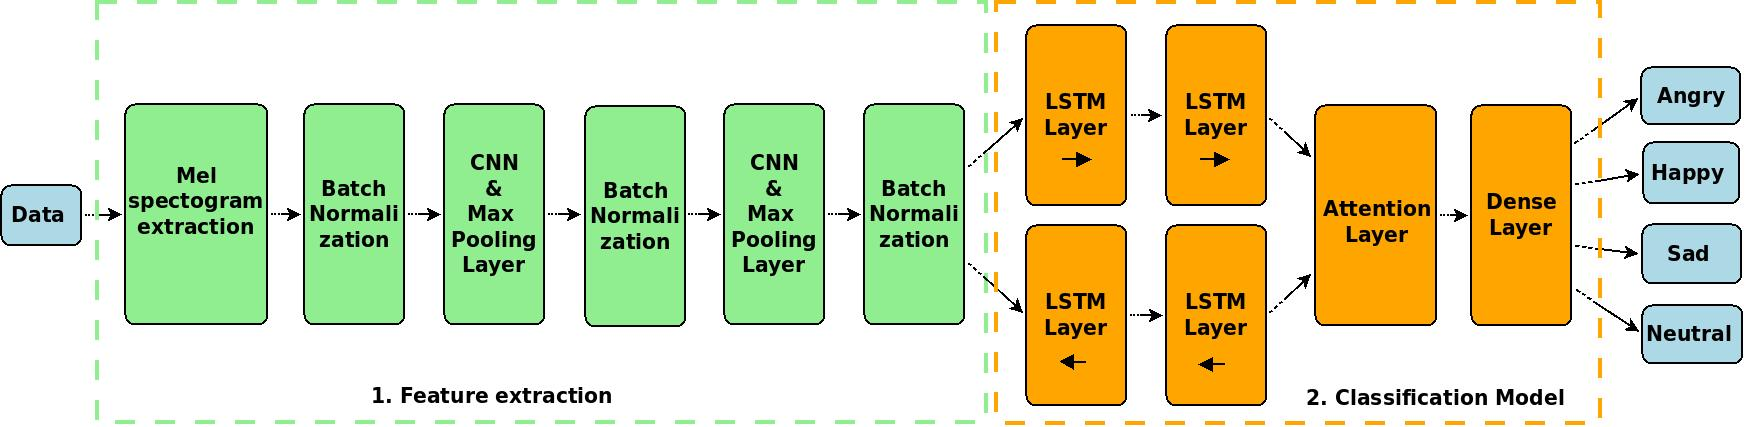
\includegraphics[scale=0.275]{Sistem_Diagram}
				\end{figure}
			Cum am mentionat si in capitolul precedent, "Speech Emotion Recognition" nu a ajuns in punctul in care poate fi pus pe piata. Astfel am decis sa fac o comparatie teoritica incercad sa prezint alte moduri de implementare prezente in cateva articole de cercetare. In continuare voi prezenta trei arhitecturi de sisteme din recunoasterea emotiei in vorbire, care sustin cateva din principalele idei pe care si eu mi-am bazat modelul. Desi prezinta unele similaritati, acestea nu pot fi comparate in mod perfect deoarece folosesc atat baze de date diferite cat si caracteristici de intrare diferite. Deoarece nu exista un mod asa zis "corect" de a construi un model SER, avantajele si dezavantajele implementarii sunt greu de identificat. \par	
	\begin{thebibliography}{9}
		\bibitem{blanton}
			Blanton, S. The voice and the emotions. Q. Journal of Speech 1, 2 (1915), 154–172.
		\bibitem{leviholler}
			Levinson SC, Holler J. 2014 The origin of human multi-modalcommunication. Phil. Trans. R. Soc. B 369:20130302.http://dx.doi.org/10.1098/rstb.2013.0302
		\bibitem{chriskirbi}
			Christiansen, M. H., \& Kirby, S. (2003). Language evolution: Consensus and controversies. Trends in Cognitive Sciences, 7(7), 300–307. https://doi.org/10.1016/S1364-6613(03)00136-0
		\bibitem{dellaert}
			Dellaert, F., Polzin, T. and Waibel, A. Recognizing emotion in speech. In Proceedings of ICSLP 3, (Philadelphia, 	PA, 1996). IEEE, 1970–1973.
		\bibitem{bjorn1}
			Bjorn W.Schuller Speech Emotion Recognition: Two Decades in a Nutshell, Benchmarks, and Ongoing Trends
		\bibitem{meld}
			S. Poria, D. Hazarika, N. Majumder, G. Naik, R. Mihalcea, E. Cambria. MELD: A Multimodal Multi-Party Dataset for Emotion Recognition in Conversation.
		\bibitem{huahu}
			Huahu, X., Jue, G., Jian, Y., 2010. Application of speech emotion recognition in intelli-
			gent household robot. In: 2010 International Conference on Artificial Intelligence and
			Computational Intelligence, 1, pp. 537–541. doi: 10.1109/AICI.2010.118
		\bibitem{gupta}
			Gupta, P. , Rajput, N. , 2007. Two-stream emotion recognition for call center monitoring.
			Proc. Interspeech 2007, 2241–2244 .
		\bibitem{szwoch}
			Szwoch, M. , Szwoch, W. , 2015. Emotion recognition for affect aware video games. In:
			Chora ś , R.S. (Ed.), Image Processing \& Communications Challenges 6. Springer Inter-
			national Publishing, Cham, pp. 227–236 .
		\bibitem{lancker}
			Lancker, D.V. , Cornelius, C. , Kreiman, J. , 1989. Recognition of emotionalprosodic mean-
			ings in speech by autistic, schizophrenic, and normal children. Develop. Neuropsy-
			chol. 5 (2–3), 207–226 .
		\bibitem{mehmet}
			Mehmet Berkehan Akçay, Kaya Oğuz, Speech emotion recognition: Emotional models, databases, features, preprocessing methods, supporting modalities, and classifiers, Speech Communication, Volume 116, 2020, Pages 56-76, ISSN 0167-6393, https://doi.org/10.1016/j.specom.2019.12.001.
		\bibitem{koolagudi}
			Koolagudi, S.G., Rao, K.S., 2012. Emotion recognition from speech: a review. Int. J. Speech Technol. 15 (2), 99–117.
		\bibitem{hcf1}
			Koolagudi, S. G., Maity, S., Kumar, V. A., Chakrabarti, S., \& Rao,	K. S. (2009). IITKGP-SESC: speech database for emotion analysis. Communications in computer and information science, LNCS.
		\bibitem{hcf2}
			Nwe, T. L., Foo, S. W., \& Silva, L. C. D. (2003). Speech emotion recognition using hidden Markov models. Speech Communication, 41, 603–623.
		\bibitem{hcf3}
			Schroder, M., \& Cowie, R. (2006). Issues in emotion-oriented computing toward a shared understanding. In Workshop on emotion and computing (HUMAINE)
			Berlin: Springer
		\bibitem{graves}
			Graves, A. \& Jaitly, Navdeep. (2014). Towards end-to-end speech recognition with recurrent neural networks. 31st International Conference on Machine Learning, ICML 2014. 5. 1764-1772. 
		\bibitem{tzir}
			Tzirakis, Panagiotis \& Trigeorgis, George \& Nicolaou, Mihalis \& Schuller, Björn \& Zafeiriou, Stefanos. 		(2017). End-to-End Multimodal Emotion Recognition Using Deep Neural Networks. IEEE Journal of Selected Topics in Signal Processing. PP.10.1109/JSTSP.2017.2764438. 
		\bibitem{misramadi}
			S. Mirsamadi, E. Barsoum and C. Zhang, "Automatic speech emotion recognition using recurrent neural networks with local attention," 2017 IEEE International Conference on Acoustics, Speech and Signal Processing (ICASSP), New Orleans, LA, 2017, pp. 2227-2231.
		\bibitem{zhang}
			Zhang, Zixing \& Wu, Bingwen \& Schuller, Björn. (2019). Attention-Augmented End-to-End Multi-Task Learning for Emotion Prediction from Speech. 
		\bibitem{yuan}
			Li, Yuanchao, Tianyu Zhao and Tatsuya Kawahara. “Improved End-to-End Speech Emotion Recognition Using Self Attention Mechanism and Multitask Learning.” INTERSPEECH 2019 (2019).
	\end{thebibliography}
\end{document}




























